\documentclass[12pt,titlepage]{article}
\usepackage[margin=1.25in]{geometry}
\usepackage{graphicx,amsmath,blindtext,minted}

%% Variables definition
\newcommand{\vSubject}{Data Structure and Algorithm Practicum}
\newcommand{\vSubtitle}{Sorting}
\newcommand{\vSubsubtitle}{Bubble, Selection, and Insertion Sort}
\newcommand{\vName}{Muhammad Baihaqi Aulia Asy'ari}
\newcommand{\vNIM}{2241720145}
\newcommand{\vClass}{1I}
\newcommand{\vDepartment}{Information Technology}
\newcommand{\vStudyProgram}{D4 Informatics Engineering}

%% [START] Tikz related stuff
\usepackage{tikz}
\usetikzlibrary{svg.path,calc,shapes.geometric,shapes.misc}
\tikzstyle{terminator} = [rectangle, draw, text centered, rounded corners = 1em, minimum height=2em]
\tikzstyle{preparation} = [chamfered rectangle, chamfered rectangle sep=0.75em, draw, text centered, minimum height = 2em]
\tikzstyle{process} = [rectangle, draw, text centered, minimum height=2em]
\tikzstyle{decision} = [diamond, aspect=2, draw, text centered, minimum height=2em]
\tikzstyle{data}=[trapezium, draw, text centered, trapezium left angle=60, trapezium right angle=120, minimum height=2em]
\tikzstyle{connector} = [line width=0.25mm,->]
%% [END] Tikz related stuff

%% [START] Fancy header related stuff
\usepackage{fancyhdr}
\pagestyle{fancy}
\setlength{\headheight}{15pt} % compensate fancyhdr style
\fancyhead{}
\fancyfoot{}
\fancyfoot[L]{\thepage}
\fancyfoot[R]{\textit{\vSubject - \vSubtitle}}
\renewcommand{\footrulewidth}{0.4pt}% default is 0pt, overline for footer
%% [END] Fancy header related stuff

%% [START] Custom tabular command related stuff
\usepackage{tabularx}
\newcommand{\details}[2]{
    #1 & #2  \\
}
%% [END] Custom tabular command related stuff

%% [START] Figure related stuff
\newcommand{\image}[3][1]{
    \begin{figure}[h]
        \centering
        \includegraphics[#1]{#2}
        \caption{#3}
        \label{#3}
    \end{figure}
}
%% [END] Figure related stuff

%%
\usepackage{pgf-umlcd}

\renewcommand{\umldrawcolor}{black}
\renewcommand{\umlfillcolor}{white}
%%

%% [BEGIN] Custom enumerator
\usepackage{enumitem}
%% [END] Custom enumerator

%% [BEGIN] Paragraph indent
\usepackage{indentfirst}
%% [END] Paragraph indent

\begin{document}
\begin{titlepage}
    \centering
    \vfill
    {\bfseries\LARGE
        \vSubject\\
        \vskip0.25cm
        \vSubtitle
        \vskip0.25cm
        \vSubsubtitle
    }
    \vfill
    
\includegraphics[width=6cm]{images/polinema-logo.png}
    \vfill
    {
        \textbf{Name}\\
        \vName\\
        \vskip0.5cm
        \textbf{NIM}\\
        \vNIM\\
        \vskip0.5cm
        \textbf{Class}\\
        \vClass\\
        \vskip0.5cm
        \textbf{Department}\\
        \vDepartment\\
        \vskip0.5cm
        \textbf{Study Program}\\
        \vStudyProgram
    }
\end{titlepage}

\newpage

\setcounter{section}{2}

\begin{enumerate}
    \item Practicum Steps
    \begin{enumerate}[label=\textbf{\alph*.}]
        \item \textbf{Practicum 1 – Create Student Class}
        \begin{enumerate}[label=\arabic*.]
            \item Pay attention in following class diagram. This will be used as our reference when creating Students Class.
            \mbox{}\\
            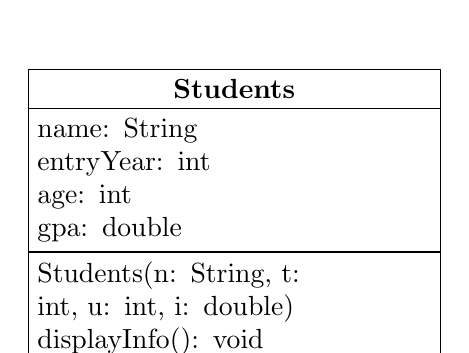
\begin{tikzpicture}
                \begin{class}[text width=5cm]{Students}{0,0}
                    \attribute{name: String}
                    \attribute{entryYear: int}
                    \attribute{age: int}
                    \attribute{gpa: double}
                    \operation{Students(n: String, t: int, u: int, i: double)}
                    \operation{displayInfo(): void}
                \end{class}
            \end{tikzpicture}
            \mbox{}\\
            \item Create \textbf{Students} class as follows!
            \begin{minted}[autogobble,breaklines]{java}
                package Sorting;

                public class Student {
                    String name;
                    int entranceYear, age;
                    double gpa;

                    public Student(String n, int y, int a, double g) {
                        name = n;
                        entranceYear = y;
                        age = a;
                        gpa = g;
                    }

                    void print() {
                        System.out.println("Name         : "+name);
                        System.out.println("Entrance Year: "+entranceYear);
                        System.out.println("Age          : "+age);
                        System.out.println("GPA          : "+gpa);
                    }
                }
            \end{minted}
        \end{enumerate}
        \item \textbf{Practicum 2 – Create HighAchieverStudent Class}
        \begin{enumerate}[label=\arabic*.]
            \item In HighAchieverStudent Class, create a list and a method to sort the student’s data based on their GPA. In addition, create a method to display all those data and other method to insert the data to the list. Take a look at class diagram below!
            \mbox{}\\
            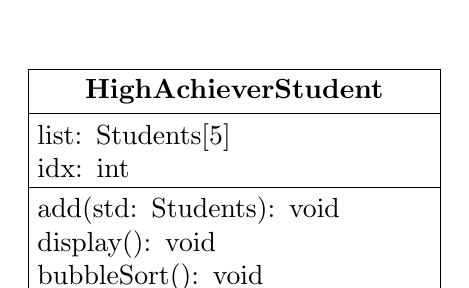
\begin{tikzpicture}
                \begin{class}[text width=5cm]{HighAchieverStudent}{0,0}
                    \attribute{list: Students[5]}
                    \attribute{idx: int}
                    \operation{add(std: Students): void}
                    \operation{display(): void}
                    \operation{bubbleSort(): void}
                \end{class}
            \end{tikzpicture}
            \mbox{}\\
            \item Create \textbf{HighAchieverStudent} class as follows!
            \begin{minted}[autogobble,breaklines]{java}
                package Sorting;

                public class HighAchieverStudent {
                    Student[] list = new Student[5];
                    int idx;
                }
            \end{minted}
            \item Add method add() in that class. This method will be used to add an object from \textbf{Students} class to listStd attribute.
            \begin{minted}[autogobble,breaklines]{java}
                void add(Student std) {
                    if (idx<list.length) {
                        list[idx] = std;
                        idx++;
                    } else {
                        System.out.println("The student list is already full-filled");
                    }
                }
            \end{minted}
            \item Add method display() in that class. This method will be used to display all the data that is exist in listStd. Take a look on how we use for loops, even though it is quite different than usual, the concept is still similar. Instead of accessing each element by its index, we just loop by each element available in the list.
            \begin{minted}[autogobble,breaklines]{java}
                void display() {
                    for (Student student : list) {
                        student.print();
                        System.out.println("------------------------ ------------------------");
                    }
                }
            \end{minted}
            \item Add method bubbleSort() in that class.
            \begin{minted}[autogobble,breaklines]{java}
                void bubbleSort() {
                    for (int i = 0; i < list.length-1; i++) {
                        for (int j = 0; j < list.length-i-1; j++) {
                            if (list[j].gpa > list[j-1].gpa) {
                                Student tmp = list[j-1];
                                list[j] = list[j-1];
                                list[j-1] = tmp;
                            }
                        }
                    }
                }
            \end{minted}
            \item Up to this point, the HighAchieverStudent class is finished
        \end{enumerate}
        \item \textbf{Practicum 3 – Create Main Class}
        \begin{enumerate}[label=\arabic*.]
            \item Create main class and its main method
            \begin{minted}[autogobble,breaklines]{java}
                public class Main {
                    public static void main(String[] args) {

                    }
                }
            \end{minted}
            \item In main method, create 2 objects from \textbf{Scanner} class, and an object from \textbf{HighAchieverStudent} class. After that, declare the variable of amountStd to 5!
            \begin{minted}[autogobble,breaklines]{java}
                Scanner s1 = new Scanner(System.in);
                Scanner s2 = new Scanner(System.in);
                HighAchieverStudent data = new HighAchieverStudent();
                int n = 5;
            \end{minted}
            \item Make loops 5 times with for, to insert name, age, entryYear, and GPA foreach students. Once it is done, instantiate the object from \textbf{Students} class and insert it to the list in \textbf{HighAchieverStudent} class.
            \begin{minted}[autogobble,breaklines]{java}
                for (int i = 0; i < n; i++) {
                    System.out.print("Name         : ");
                    String name = s2.nextLine();
                    System.out.print("Entrance year: ");
                    int year = s1.nextInt();
                    System.out.print("Age          : ");
                    int age = s1.nextInt();
                    System.out.print("GPA          : ");
                    int gpa = s1.nextInt();

                    Student s = new Student(name, year, age, gpa);
                    data.add(s);
                }
            \end{minted}
            \item Display the student’s data that has been inserted in the list!
            \begin{minted}[autogobble,breaklines]{java}
                System.out.println("Unsorted student list:");
                data.display();
            \end{minted}
            \item Call method bubbleSort() and show the result!
            \begin{minted}[autogobble,breaklines]{java}
                System.out.println("Student data after sorted in decending order in gpa: ");
                data.bubbleSort();
                data.display();
            \end{minted}
            Try to execute the program and understand the result. Are the data in the list is sorted based on GPA?
        \end{enumerate}
        \item \textbf{Practicum 4 – Add Selection Sort process in HighAchieverStudent Class}
        \begin{enumerate}[label=\arabic*.]
            \item Go to \textbf{HighAchieverStudent} class, add method selectionSort() there. This method will do the sorting process in ascending order, but with selection sort approach.
            \begin{minted}[autogobble,breaklines]{java}
                void selectionSort() {
                    for (int i = 0; i < list.length-1; i++) {
                        int idxMin = i;
                        for (int j = i+1; j < list.length; j++) {
                            if (list[j].gpa < list[idxMin].gpa) {
                                idxMin = j;
                            }
                        }
                        Student tmp = list[idxMin];
                        list[idxMin] = list[i];
                        list[i] = tmp;
                    }
                }
            \end{minted}
            \item After that, open main class. In main method, add these line of code to execute selectionSort() method that we’ve just created. Try to execute the program and understand the result. Are the data in the list is
            \begin{minted}[autogobble,breaklines]{java}
                System.out.println("Ascending Sorted student list");
                data.selectionSort();
                data.display();
            \end{minted}
            sorted based on GPA?
        \end{enumerate}
        \item \textbf{Practicum 5 – Add Insertion Sort process in HighAchieverStudent Class}
        \begin{enumerate}[label=\arabic*.]
            \item Go to \textbf{HighAchieverStudent} class, add method insertionSort() there. This method will do the sorting process in ascending order, but with selection sort approach.
            \begin{minted}[autogobble,breaklines]{java}
                void insertionSort() {
                    for (int i = 0; i < list.length-1; i++) {
                        Student temp = list[i];
                        int j = i;
                        while (j > 0 && list[j-1].gpa > temp.gpa) {
                            list[j] = list[j-1];
                            j--;
                        }
                        list[j] = temp;
                    }
                }
            \end{minted}
            \item After that, open main class. In main method, add these lines of code to execute insertionSort () method that we’ve just created.
            \begin{minted}[autogobble,breaklines]{java}
                System.out.println("Ascending Sorted student list");
                data.insertionSort();
                data.display();
            \end{minted}
            Try to execute the program and understand the result. Are the data in the list is sorted based on GPA?
        \end{enumerate}
    \end{enumerate}
    \item \textbf{Questions}
    \begin{enumerate}[label=\arabic*.]
        \item In which class we have a function to do sorting with bubble sort approach?
        \mbox{}\\
        \texttt{Answer: }
        \mbox{}\\
        HighAchieverStudent
        \item In which class we have a function to do sorting with insertion sort approach?
        \mbox{}\\
        \texttt{Answer: }
        \mbox{}\\
        HighAchieverStudent
        \item What is the meaning of swapping process? Write the code to do the swapping process in the program above!
        \mbox{}\\
        \texttt{Answer: }
        \mbox{}\\
        its a process where the program switch an element of an array with another element in the same array. usually use for sorting.
        \item In bubbleSort(), there is these lines of code, what’s the function of it?
        \begin{minted}[autogobble,breaklines]{java}
            if (list[j].gpa > list[j-1].gpa) {
                Student tmp = list[j-1];
                list[j] = list[j-1];
                list[j-1] = tmp;
            } 
        \end{minted}
        \mbox{}\\
        \texttt{Answer: }
        \mbox{}\\
        if the previous element of the array is smaller than the current array, the program will swap the element.
        \item Look at the loops inside the bubbleSort() method:
        \begin{minted}[autogobble,breaklines]{java}
            for (int i = 0; i < list.length-1; i++) {
                for (int j = 0; j < list.length-i-1; j++) {

                }
            }
        \end{minted}
        \begin{enumerate}[label=\alph*.]
            \item What’s the difference of loop i and loop j?
            \mbox{}\\
            \texttt{Answer: }
            \mbox{}\\
            the j loop iterate through the array to swap and carry. and the i loop iterate the starting index for the swap and carry process. 
            \item Why is the criteria of loop i is i<listStd.length-1?
            \item \mbox{}\\
            \texttt{Answer: }
            \mbox{}\\
            because the i doesnt need to iterate through the last element.
            \item Why is the criteria of loop j is j<listStd.length-i?
            \mbox{}\\
            \texttt{Answer: }
            \mbox{}\\
            because the program doesnt need to swap through the whole array when the end part of the array is alredy sorted. 
            \item If the data in listStd is 50, how many loop i will happen? And how many bubble sort steps will be?
            \mbox{}\\
            \texttt{Answer: }
            \mbox{}\\
            the i loop would need to loop through the same amount of data in the array, which is 50. and the swap and carry process would need to be processed in amount of the sum of series of number from 1 to the amount of data in the array.
        \end{enumerate}
        \item In selection sort method, there is these lines of code, what’s that for?
        \begin{minted}[autogobble,breaklines]{java}
            int idxMin = i;
            for (int j = i+1; j < list.length; j++) {
                if (list[j].gpa < list[idxMin].gpa) {
                    idxMin = j;
                }
            }
        \end{minted}
        \mbox{}\\
        \texttt{Answer: }
        \mbox{}\\
        it loops through the unsorted part of the array and then saving the index of the minimum value in the array. 
        \item Change the insertionSort method so that the user has options to sort in either ascending or descending order. You can do it by adding a parameter, and this parameter’s value will be assigned through function calling in main class
        \begin{minted}[autogobble,breaklines]{java}
            void insertionSort(boolean asc) {
                for (int i = 0; i < list.length-1; i++) {
                    Student temp = list[i];
                    int j = i;
                    if(asc) {
                        while (j > 0 && list[j-1].gpa > temp.gpa) {
                            list[j] = list[j-1];
                            j--;
                        }
                    } else {
                        while (j > 0 && list[j-1].gpa < temp.gpa) {
                            list[j] = list[j-1];
                            j--;
                        }
                    }
                    list[j] = temp;
                }
            }
        \end{minted}
    \end{enumerate}
    \item \textbf{Assignment}
    \begin{enumerate}[label=\arabic*.]
        \item There is a company that provide services in airplane ticket sales, they are developing a backend system for ticket reservation. One of its features is to display all available tickets based on filter from user. The ticket list must able to be sorted by the price in ascending and descending order. Implement these class diagrams in java program and create the sorting algorithm with \textbf{bubble sort} and \textbf{selection sort}
        \mbox{}\\
        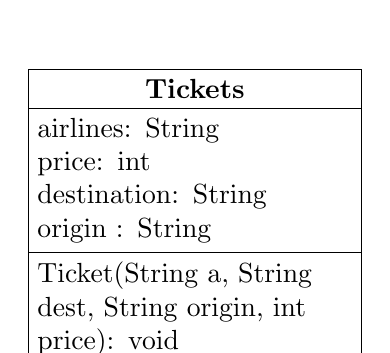
\begin{tikzpicture}
            \begin{class}[text width=4cm]{Tickets}{0,0}
                \attribute{airlines: String}
                \attribute{price: int}
                \attribute{destination: String}
                \attribute{origin : String}
                \operation{Ticket(String a, String dest, String origin, int price): void}
            \end{class}
        \end{tikzpicture}
        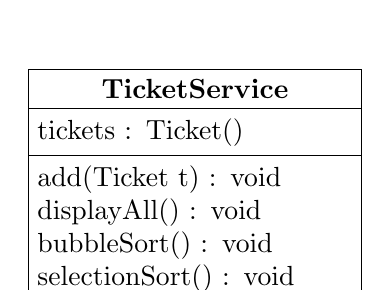
\begin{tikzpicture}
            \begin{class}[text width=4cm]{TicketService}{0,0}
                \attribute{tickets : Ticket()}
                \operation{add(Ticket t) : void}
                \operation{displayAll() : void}
                \operation{bubbleSort() : void}
                \operation{selectionSort() : void}
            \end{class}
        \end{tikzpicture}
        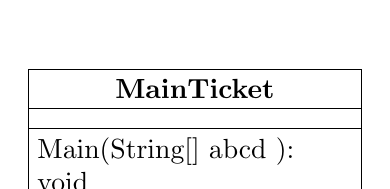
\begin{tikzpicture}
            \begin{class}[text width=4cm]{MainTicket}{0,0}
                \attribute{}
                \operation{Main(String[] abcd ): void}
            \end{class}
        \end{tikzpicture}
        \mbox{}\\
        \begin{minted}[autogobble,breaklines]{java}
            package Assignment1;

            public class Tickets {
                String airlines, destination, origin;
                int price;

                public Tickets(String a, String dest, String origin, int price) {
                    airlines = a;
                    destination = dest;
                    this.origin = origin;
                    this.price = price;
                }
            }
        \end{minted}
        \begin{minted}[autogobble,breaklines]{java}
            package Assignment1;

            public class TicketService {
                Tickets[] tickets = new Tickets[1];

                public void add(Tickets t) {
                    if (tickets[0] == null) {
                        tickets[0] = t;
                    } else {
                        Tickets[] temp = tickets;
                        int newTicketsLen = tickets.length + 1;
                        tickets = new Tickets[newTicketsLen];

                        for (int i = 0; i < temp.length; i++) {
                            tickets[i] = temp[i];
                        }

                        tickets[newTicketsLen-1] = t;
                    }
                }

                public void displayAll() {
                    for (int i = 0; i < tickets.length; i++) {
                        System.out.println("------------------------ ------------------------");
                        System.out.printf("%s Airlines\n",tickets[i].airlines);
                        System.out.printf("From %s to %s\n",tickets[i].origin, tickets[i].destination);
                        System.out.printf("Cost: Rp %,d\n",tickets[i].price);
                    }
                }

                void bubbleSort(boolean asc) {
                    for (int i = 0; i < tickets.length-1; i++) {
                        for (int j = 0; j < tickets.length-i-1; j++) {
                            if (asc) {
                                if (tickets[j].price > tickets[j-1].price) {
                                    Tickets tmp = tickets[j-1];
                                    tickets[j] = tickets[j-1];
                                    tickets[j-1] = tmp;
                                }
                            } else {
                                if (tickets[j].price < tickets[j-1].price) {
                                    Tickets tmp = tickets[j-1];
                                    tickets[j] = tickets[j-1];
                                    tickets[j-1] = tmp;
                                }
                            }
                        }
                    }
                }

                void selectionSort(boolean asc) {
                    for (int i = 0; i < tickets.length-1; i++) {
                        int idxSelected = i;
                        for (int j = i+1; j < tickets.length; j++) {
                            if (asc) {
                                if (tickets[j].price < tickets[idxSelected].price) {
                                    idxSelected = j;
                                }
                            } else {
                                if (tickets[j].price > tickets[idxSelected].price) {
                                    idxSelected = j;
                                }
                            }
                        }
                        Tickets tmp = tickets[idxSelected];
                        tickets[idxSelected] = tickets[i];
                        tickets[i] = tmp;
                    }
                }
            }
        \end{minted}
        \begin{minted}[autogobble,breaklines]{java}
            package Assignment1;

            public class MainTicket {
                public static void main(String[] args) {
                    
                }
            }
        \end{minted}
        \item Premiere League in 2020 is already in half-season. In this season, Liverpool is the top of the list, the full list is displayed below
        \mbox{}\\
        \begin{center}
            \includegraphics[width=7cm]{images/figures/fig1.png}
        \end{center}
        \mbox{}\\
        Change the standings list above to class diagram that has sorting club function based on highest to smallest points (in ascending order) with insertion sort algorithm. Take these following class diagrams as your reference:
        \mbox{}\\
        \texttt{Answer: }
        \mbox{}\\
        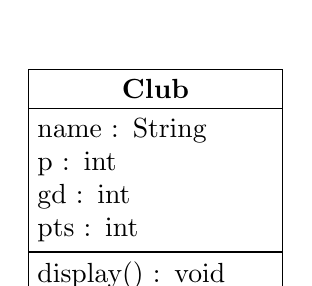
\begin{tikzpicture}
            \begin{class}[text width=3cm]{Club}{0,0}
                \attribute{name : String}
                \attribute{p : int}
                \attribute{gd : int}
                \attribute{pts : int}
                \operation{display() : void}
            \end{class}
        \end{tikzpicture}
        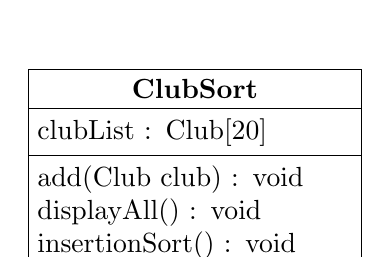
\begin{tikzpicture}
            \begin{class}[text width=4cm]{ClubSort}{0,0}
                \attribute{clubList : Club[20]}
                \operation{add(Club club) : void}
                \operation{displayAll() : void}
                \operation{insertionSort() : void}
            \end{class}
        \end{tikzpicture}
        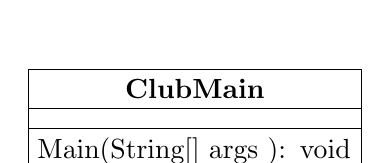
\begin{tikzpicture}
            \begin{class}[text width=4cm]{ClubMain}{0,0}
                \attribute{}
                \operation{Main(String[] args ): void}
            \end{class}
        \end{tikzpicture}
        \mbox{}\\
    \end{enumerate}
\end{enumerate}

\end{document}